\problemname{Snömur}
Efter förnedringen i snöbollskriget tänker Sverige bygga en snömur, och tvinga Finland att betala för den.
Muren ska ha en viss bredd $W$, och vara så hög som möjligt (it's going to be \emph{yuuuge}!).

Som byggmaterial finns det ett antal snöblock som alla har höjden 1, men kan ha olika bredder.
När muren konstrueras måste varje block uppfylla följande en regel: på raden under blocket,
på de två positioner blocker har sina ändpunkter, måste det ligga ett block precis till höger och vänster om punkten,
undantaget början och slutet på en rad, där det istället måste finnas en ändpunkt \emph{på varje rad}.

Följande bild illustrerar några otillåtna (vänster) och tillåtna (höger) murar:

\begin{figure}[h]
	\centering
	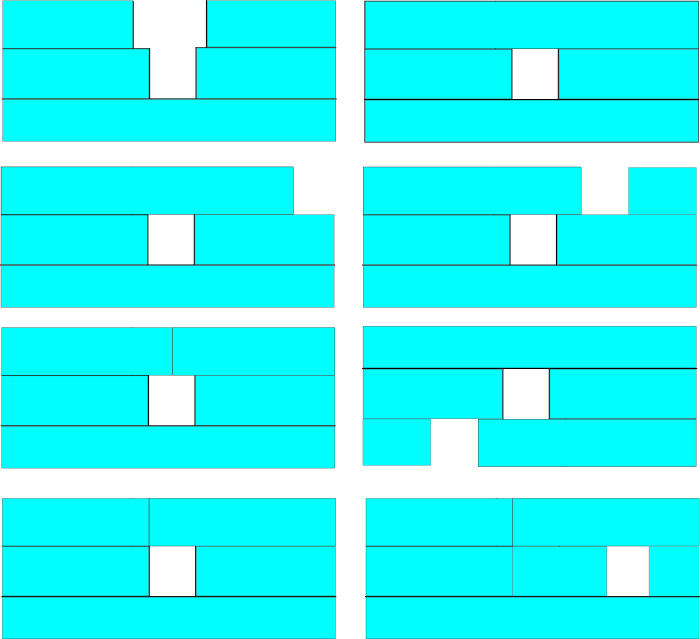
\includegraphics[width=0.7\textwidth]{mur.png}
	\caption{Ett antal otillåtna (vänster) och tillåtna (höger) murar.}
\end{figure}

Givet bredden $W$ och de möjliga blocken, konstruera en så hög mur som möjligt.

\section*{Indata}
Den första raden innehåller tre heltal heltal $T$, $N$ och $W$ - testfallets nummer, antalet block och bredden på muren.
Nästa rad innehåller $N$ heltal, bredden på varje block.

% TODO
Du kan ladda ner alla testfall \url{HÄR}.

\section*{Utdata}
På den första raden ska du skriva ut höjden på din mur, $H$.

Du ska sedan skriva ut $H$ rader, en för varje rad i din mur.
Rad $i$ ska först ha ett tal $B$, antalet block på den raden i din mur.
Detta ska följas av $B$ par av heltal $P_{i,j} L_{i,j}$ positionen och längden för det $j$:te blocket på raden.

\section*{Inskickning}
När du skickar in din lösning räcker det med ett program som läser in testfallets nummer $T$ och skriver ut lösningen för det testfallet.
% TODO
Om du inte vill skriva ett sådant program själv kan du använda en sida vi konstruerade: \url{HÄR} där du kan klistra in
alla dina lösningar och få ett Python 3-program som du kan skicka in.

\section*{Poängsättning}
Antag att på ett testfall värt $P$ poäng så får ditt program höjden $X$, och det bästa programmet höjden $Y$. Då får du $P \times \frac{X}{Y}$ poäng.

Innan tävlingsslut kommer alla lösningar rättas med $Y = 2 \times \frac{\sum{\text{höjder}}}{W}$

Totalt finns 10 testfall, och varje testfall kan ge upp till 10 poäng.
